% chapter 4
\cleardoublepage
\phantomsection
\chapter{Implementation and Testing}
Design complete with research in hand, I am now ready to begin implementation. I intend on completing this process in three distinct stages: virtual hardware creation \& configuration, guest software configuration and lastly custom software creation.

I expect the first two stages should complete without much upset and can probably done in a nonrepetative fashion for the most part. The last stage has additional sufficient complexity and uniqueness that leads me to conclude this part of the process will almost definitely end up being considerably more iterative in nature.

Once implementation has been achieved, I will test my system by running my program multiple times under increasing node counts. This process will be outlined in more detail in the second section of this chapter.

\section{Implementing a Beowulf cluster: Configuring and preparing}

\textbf{\sffamily{Setting up and configuring the virtual switch \& nodes}}

The first step I am taking in setting up and configuring my cluster is hardware preparation. Specifically, I need to make sure the network stack on the hypervisor is up to the task I will be setting for it. As set forth in my design document, the Beowulf cluster I am building will have its own dedicated switch away from the main home network to reduce packet impedance and collision.

To configure a second virtual switch on my hypervisor, I will need to modify the interfaces file found in the Debian file system running on the host. Within, I am adding a carbon copy block from the original virtual switch (`bridge').

\lstinputlisting[numbers=right,breaklines=true,tabsize=2,language=]{CITY3111/additionals/text/interfaces_snip.txt}
\begin{center}
    \emph{Live snip from my interfaces file}
\end{center}
\vfill\break

The only major changes one can see between the original virtual switch (`vmbr0') and the new virtual switch (`vmbr1`) are the changes in the address subnets used between switches and the absence of a physical network port or gateway on the new switch as these features are not required in this particular usecase.

After a reboot, the hypervisor will recognise and auto-configure the network switch and make it available for use. When it comes to configuring the virtual machines, the only step that will be required is to configure the preconfigured virtual network interface cards (NICs) to use an IP on the same subnet as the host. Routing will be handled by the RIP protocol without additional instruction.

Network configuration complete, the other step required in the virtual hardware configuration stage is to create the virtual guests. In Proxmox VE, this is completed within the GUI.

On creation of a virtual machine, both in Proxmox VE and most other hypervisors, a wizard presents itself to step the user though various configuration options. This is ideal for my usecase as I can use the options decided upon during the design stage of this project to optimise my cluster for performance.

\begin{figure}[H]
    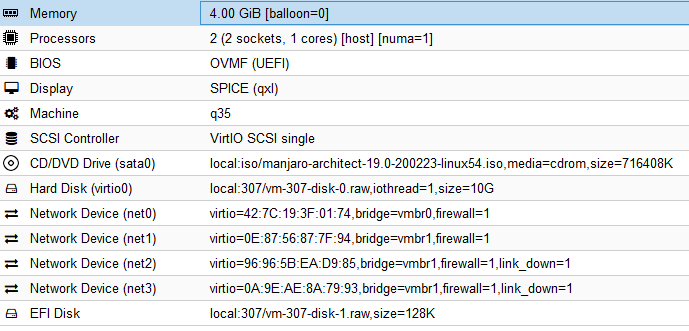
\includegraphics[width=\linewidth]{CITY3111/bitmaps/figure_10.png}
    \caption{Screenshot of guest OS hardware configuration}
    \label{figure_10}
\end{figure}

As seen in the screenshot above, the end configuration is geared as best as it possibly can be for optimum performance. All network adaptors and drives are connected to the VirtIO bus, a generous memory count has been allocated and an up-to-date BIOS and chipset is being simulated.

With the primary node configured, cloning of the configuration is completed by using the hypervisor's build-in cloning tool. Hard disk cloning will be done at a later point once the operating system has been fully configured and is ready for the custom software package.

\textbf{\sffamily{Setting up and configuring the guest OS: Setup}}

With my virtual guest machine booted and confirmed functional, the next stage was to install Manjaro using the Architect installer. Manjaro's Architect installer allows full customisation over what packages and features get installed to the system initially. To avoid bloat, I will be keeping the master image as minimal as possible.

On initial boot of the ISO, I am presented a series of questions including what timezone I wish to use, the language and keyboard settings I wish to use and the driver suite I would like to choose. Naturally, regional questions will be set to British English in this case and require no further explanation, however the driver suite I want to use is worth additional discussion.

Linux drivers typically tend to what are referred to as `free' drivers. Free drivers are any drivers that are based wholly on free and open-source software (FOSS). As a FOSS OS, Linux usually has a free driver for every major brand and kind of PC hardware available and in my system this is no exception. The only hardware that might be unusual in this virtual environment is the VirtIO suite of devices.

Upon deeper inspection of the VirtIO device suite, it has become apparent to me that it is in fact part of the Linux KVM module which is in turn included in the Linux kernel. Source code is available via the Linux kernel repositories. This means that I can boot with free drivers and not lose functionality or performance in my system. Addendum to that, the Spice GPU and driver are not fundamental to the performance of a CLI-based OS and can be suitably supported by the basic Linux video driver suite.

Once the system has been booted, the installer automatically starts a shell with root permissions. My first job is to populate pacman's key-ring and launch the setup process. To do this, I ran three commands listed below.

\lstinputlisting[numbers=left,breaklines=true,tabsize=2,language=]{CITY3111/additionals/text/setup-launch.txt}
\begin{center}
    \emph{Pre-setup commands}
\end{center}

Within the setup, I am met with numerous options, many of which do not necessarily apply to me. To keep this write-up as simple as possible I will explain only the steps that apply to me, starting with disc partitioning. Architect offers automatic partitioning as a preparatory option, however this involves creating a swap drive which, once configured, is difficult to modify.As I have mentioned, I may want to modify the amount of RAM I allocate to each of my nodes. This is much easier to do by creating a swap file on the root partition instead.

My best option is therefore to create my own partition table using the `cgdisk' utility. My partition table needs to account for an EFI boot volume, of which I will allocate 35 MB of space for. The rest of the disc becomes my root partition where the operating system will reside.
\vfill\break

\begin{figure}[H]
    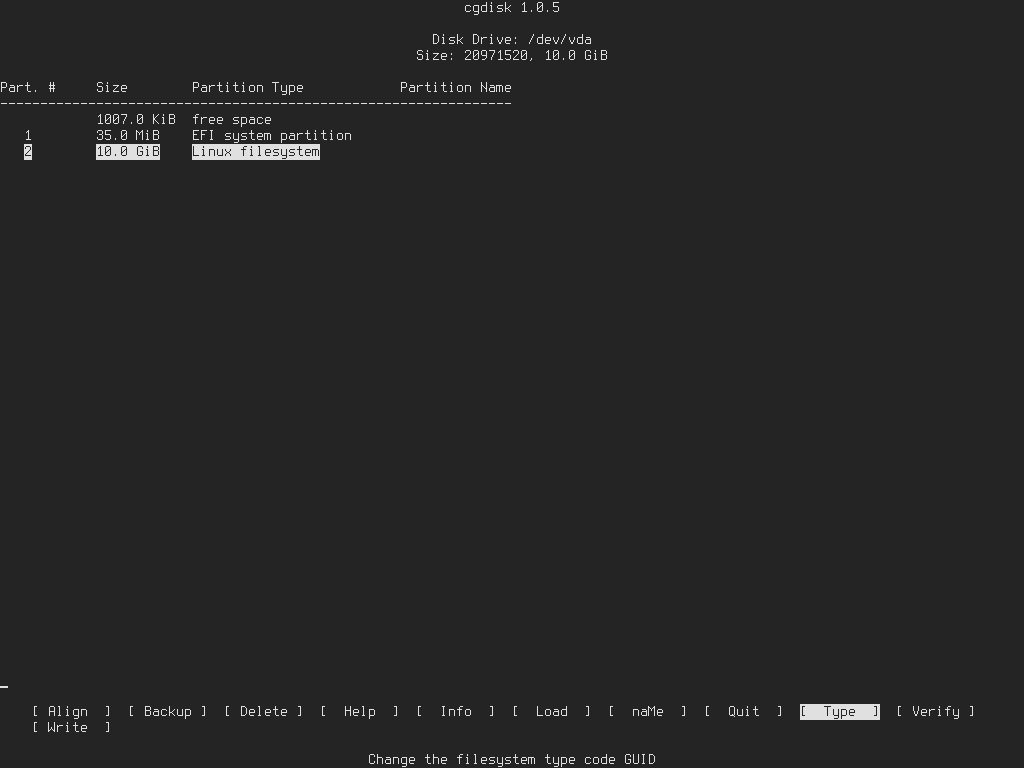
\includegraphics[width=\linewidth]{CITY3111/bitmaps/figure_11.png}
    \caption{Screenshot of completed `cgdisk' process}
    \label{figure_11}
\end{figure}

Partition table created and file systems applied, the next step is to mount the partitions at their correct locations prior to installation. Architect has a wizard which helps with this process, all I am required to do is carefully ensure I select the correct mount points for the relevant volumes. The same wizard has also allowed me to create a swapfile on the root partition and has added it to the `/etc/fstab' file which manages partition mounting on boot.

With the hard discs ready, I am in a position to begin the installation process for Manjaro. Before I can start customising my setup however, I need to install the base packages. The wizard process for this step asks some basic questions such as which kernels to use and what development packages you would like if required. For this stage, I chose the latest stable kernel (v5,4) and the base-devel package for installation. I also chose to install kernel-headers with free drivers. This whole process took approximately two minutes.

After completing the base system installation, I'm now ready to install a bootloader. This step is mandatory if I want to be able to boot the operating system once I am finished with setup. Architect offers the `refind' bootloader typically used to install Linux on older Mac machines as well as the `systemd-boot' module, however most Linux installations nowadays use the `grub2' bootloader as it is well-developed and ``just works''. This is the option I am choosing.

\begin{figure}[H]
    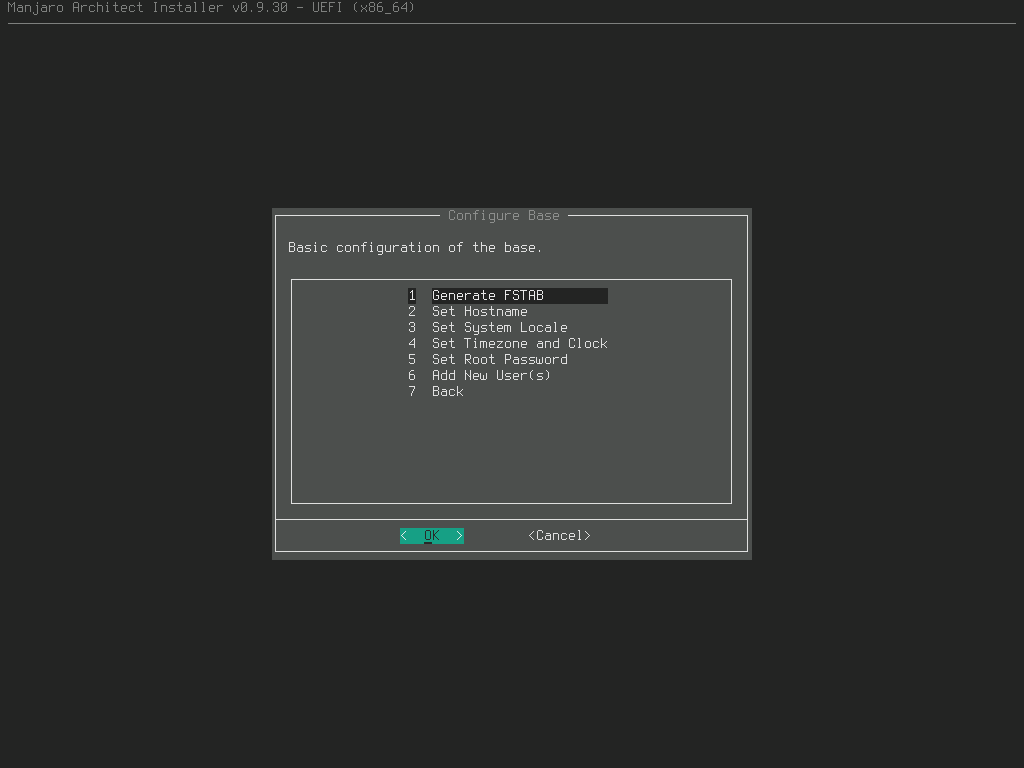
\includegraphics[width=\linewidth]{CITY3111/bitmaps/figure_12.png}
    \caption{Screenshot of base configuration menu}
    \label{figure_12}
\end{figure}

Once the bootloader is installed, the final stage in Architect's setup process I will be making use of is the base configuration. These steps, supposedly meant to be done in order, will prepare the system for general usage. While most of these steps are unimportant, there are three specific steps which I need to discuss.

The first, the system host-name, will henceforth become `CITY3111-VM\emph{n}' where \emph{n} represents the node number one-counting. This value will be important going forward, and will ultimately end up being unique per-system. Without this value being correctly configured or non-unique on the network, inter-nodal communications will be impossible.

The second step is setting the root password. I will need to set this to something secure as the root user ultimately has full power in Linux to do as it pleases. Once my regular user has sufficient super user access, I will disable logon to root with a password for security reasons.

The final step I am configuring is a new user account. Creating a user account on Architect is slightly more involved than just setting the password on root as it requires a decision on the user shell in use. While `bash' is the typical Linux shell, `zsh' is gaining popularity on other UNIX and UNIX-like OSes. I have experience using `zsh' so this is the shell I am choosing. After entering a password, setup informs me the user is ready for use on the next boot.

\begin{figure}[H]
    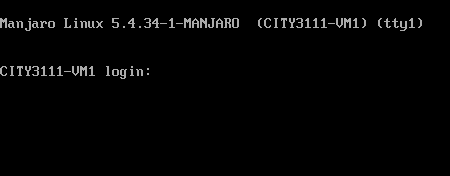
\includegraphics[width=\linewidth]{CITY3111/bitmaps/figure_13.png}
    \caption{Screenshot of fully booted Manjaro system}
    \label{figure_13}
\end{figure}

Rebooting concludes the setup portion of this section, where I have installed Manjaro using minimal settings via the Architect setup and configured a user for login. The next stage is to install the packages I need and configure the system so it is suitable for use with any custom software I wish to write and compile.

\textbf{\sffamily{Setting up and configuring the guest OS: Configuration}}

With my guest OS installed and booted and my root user logged in, the first step I need to undertake is a full OS upgrade check. This process is handled by Manjaro's package manager, `pacman'. The -Syuu flag will synchronise the system's package database with the package database found at the nearest Manjaro mirror and offer to install any upgrades found.

\lstinputlisting[numbers=right,breaklines=true,tabsize=2,language=]{CITY3111/additionals/text/pacman-syuu.txt}
\begin{center}
    \emph{Output of the `pacman -Syuu' command}
\end{center}

As is typical with fresh installs of many Linux distros, the system was already up-to-date, however it is still best practice to ensure the local database is in sync with the local mirror to greatly reduce the likelihood of attempting to get an out-of-date package. Going forward, I will install packages only using the `-S' flag with pacman to speed up the sync process.

Package database up-to-date, I am ready to begin installing software. The very first package I want to install is `sudo' which allows for protected super user access from non-root users. Sudo is considered more secure than consistent use of the root user as it only affords the target process elevation rather than the entire session. To install this, I ran `pacman -S sudo'.

With `sudo' installed, the last two steps in allowing my user super user access are to add my user to the `wheel' group and allow said group sudo access. To begin with, I add my user to the group by running `usermod -a -G wheel axessta'. With the user now in the required group, I lastly modify the `/etc/sudoers' group using the `nano' command.

\lstinputlisting[numbers=left,breaklines=true,tabsize=2,language=]{CITY3111/additionals/text/sudoers.txt}
\begin{center}
    \emph{Snipped contents of the `/etc/sudoers' file}
\end{center}

Once this step has been completed, I can test my user's permissions by logging out of the system and back in with the regular user. If the process has been completed successfully, I should be able to edit the `/etc/shadow' file using `sudo nano /etc/shadow'. I found the `usermod' command to be unreliable, and it took several runs for the system to register my user as a sudoer. I am unsure if this issue is directly related to `usermod' or if `sudo' incurs a delay either through a bug or by design, however eventually this process worked and I could modify the root user.

With functional sudo access, password-based login to the root user is no longer a desirable trait of my operating system so I wish to disable it. To do so, I need to delete the text hash for my root's user and replace it with an asterisk. In Linux's `shadow' authentication process, an asterisk is seen as an active user without password privileges, while an exclamation point is seen as a disabled user, double-exclamation point as a blocked user and a blank field as password-free access. For my purposes, an asterisk is suitable as there may be times I still want to access the root user using `sudo su root'.

\lstinputlisting[numbers=right,breaklines=true,tabsize=2,language=]{CITY3111/additionals/text/shadow.txt}
\begin{center}
    \emph{Snipped contents of the `/etc/shadow' file}
\end{center}

With a super user configured, my next logical step is to configure a static network addressing structure based on the framework specified in my Design chapter. My node featured four adaptors as seen in Figure 4,1,1, labelled ens18-21. It would therefore be logical to assume that end18 mapped to my active connection through to `vmbr0' and ens19 mapped to `vmbr1'.

To configure the adaptors I used the `systemd-network' configuration method standard in Arch Linux. With `ens18', I need to ensure a suitable connection to the landline is maintained so I will include DNS and gateway configuration details. With `ens19', only a suitable subnet and address was required to facilitate inter-nodal talks.

\lstinputlisting[numbers=right,breaklines=true,tabsize=2,language=]{CITY3111/additionals/text/systemd-network-18.txt}
\begin{center}
    \emph{Full contents of the `/etc/systemd/ens18.network' file}
\end{center}

\lstinputlisting[numbers=left,breaklines=true,tabsize=2,language=]{CITY3111/additionals/text/systemd-network-19.txt}
\begin{center}
    \emph{Full contents of the `/etc/systemd/ens19.network' file}
\end{center}

With a super user configured and the network functioning, I now need to install my packages. As I may require the ability to download additional files directly from the web, I will install `wget'. As well as this, I will be cloning files from my repository so `subversion' is another dependency for my project. Lastly, I will install the Open MPI package which, on Arch, includes the runtime and compiler.

To install these scripts, I made use of the `-S' pacman flag which synchronises the target package with the external mirror service as well as the `--noconfirm' flag which installs a package without requiring keyboard input. Additionally, I chose to enable the `sshd' service with systemd so I could initiate SSH communications between nodes. It is worth noting here however that once I clone my other nodes the SSH package will need new certificates in order to avoid insecurities and certificate clashing.

\lstinputlisting[numbers=left,breaklines=true,tabsize=2,language=]{CITY3111/additionals/text/pacman-install-script.txt}
\begin{center}
    \emph{Live snip of my `pacman' commands}
\end{center}

The last step I am able to complete uniformly on the master which can be passed evenly amongst the nodes without major reconfiguration is the hosts file. The hosts file keeps a local list of hostnames associated with IP addresses, a bit like how a DNS server would distribute domain names to clients over TCP/IP without the need for an external server. This will be useful as I won't need to manually type out IP addresses each time I wish to change the node I am connected to.

To achieve this, all I need to do is list the IPs of each node in order and the associated hostname, divided by a tabulator.

\lstinputlisting[numbers=right,breaklines=true,tabsize=2,language=]{CITY3111/additionals/text/hosts.txt}
\begin{center}
    \emph{Full contents of `/etc/hosts' file}
\end{center}

\textbf{\sffamily{Setting up and configuring the guest OS: Cloning \& Tidy-up}}

With my operating system now fundamentally ready for service, the last step I need to undertake is cloning and tidy-up. I expect this to be a four-pronged attack, with the the notable stages being cloning, renaming, re-addressing and re-certification.

For each of these steps, I will demonstrate how the process is completed on one node. Please bare in mind that the process is in fact going to be completed on the four additional nodes in sequence.

Firstly, I need to clone my master node out into the four other nodes. In Proxmox VE, a wizard is available which will automatically handle file replication and configuration matching. In the past I have found this option to be reliable so I will utilise it today.
\vfill\break

\begin{figure}[H]
    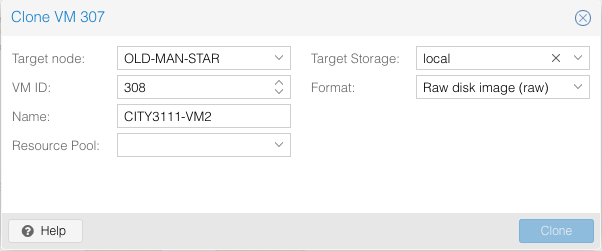
\includegraphics[width=\linewidth]{CITY3111/bitmaps/figure_14.png}
    \caption{Screenshot of VM cloning using Proxmox VE}
    \label{figure_14}
\end{figure}

The wizard takes approximately five minutes to complete per node and, once done, boots the newly created node for you. As we currently have two nodes with conflicting preconfigured hostnames and IP addresses, I promptly halted each node in turn to avoid problems arising.

With the nodes clones, I now completed the following steps on each node in turn, always with the master node offline.

Now my nodes all exist and are accounted for, I proceeded to move onto the next stage which is renaming. To rename a system running Linux, two values must be altered. The first value is the associated hostname found on line one of `/etc/hosts' and the second is the contents of `/etc/hostname'.

Taking the `/etc/hosts' example from above first, one can see the last string on line one is `CITY3111-VM1'. For node two, this will become `CITY3111-VM2' and so on. Within `/etc/hostname', the same rule applies except the entire contents of the file must contain only our new system name.

Moving on to re-addressing of the system, this stage is essentially just as simple as the previous. All I am required to do is modify the two files I created in `/etc/systemd/network` and increment each node by one from its neighbour. For example, the IPv6 addresses of node one, which are `2001:470:1f1d:ef5:3::7' and `2001:56::5', become `2001:470:1f1d:ef5:3::8' and `2001:56::6' and so on.

With these two steps complete, a reboot of each node has ensured the systems are configured correctly and no IPs are overlapping. I have proven this by pinging the 1.1.1.1 and 192.16.56.1 IPs from all nodes simultaneously. If there were any hostname or IP address overlaps, one or more of the nodes would fail to connect to the network(s) and the pings would fail.

I am now ready to complete the final step, which is to regenerate the SSH keys for each node. While this step is somewhat optional and rarely causes issues, it will increase the security of my system and avoid certificate clashes which can happen with certain SSH clients or environments.

To renew the SSH certificates, I need to stop the `sshd' service, remove and regenerate the SSH certificates and restart the service. To make this process faster, I wrote a basic shell script to do the job for me.

\lstinputlisting[numbers=right,breaklines=true,tabsize=2,language=]{CITY3111/additionals/text/ssh-regen-sh.txt}
\begin{center}
    \emph{Full contents of `ssh-regen.sh' file}
\end{center}
\vfill\break

A correct start of SSH demonstrates the service is online and running. The final, short stage of the cluster's preparatory cycle is to copy my SSH keys between nodes.

\textbf{\sffamily{Setting up and configuring the guest OS: Exchanging SSH keys between nodes}}

With SSH now online and running across all nodes, I finally come to the final portion of this chapter which is  the exchanging of SSH keys. In order for SSH to authenticate without prompting for a password -- a prerequisite of MPI -- I need to create a public and private key pair and ensure each node has the public key for the master.

This means that the master will be able to initiate SSH connections on demand without prompting the user for a password on connection. To achieve this process, I will run the command below and answer the prompt with default values:

\lstinputlisting[numbers=left,breaklines=true,tabsize=2,language=]{CITY3111/additionals/text/ssh-keydist-sh.txt}
\begin{center}
    \emph{Single-line command}
\end{center}

This command will generate a key pair, however it has not yet left the local machine. In order to duplicate it across all nodes, I need to run the following:

\lstinputlisting[numbers=left,breaklines=true,tabsize=2,language=]{CITY3111/additionals/text/ssh-keydist-sh2.txt}
\begin{center}
    \emph{Single-line command}
\end{center}

Please bear in mind that the hostname must be changed for each new target node. Once this step has been completed, my cluster can now freely communicate whenever a master node initiates a new node call.
\vfill\break

\section{Implementation and Testing: Creating my custom software}
With my cluster environment configured, I am ready to program for the MPI runtime. To do this, I intend on compiling two programs. The first is a basic hello world program \cite{barrett_et_al_2006} which I will use to test my cluster functions as intended and all nodes respond to commands. The second program is a currently abstract custom software suite which will brute-force the eggholder function, as discussed in Chapter 3.

I hope this process to be a straight-forward one, however there is a high likelihood I may need to iterate my program several times in order to get it to work as I intend before I can conclude this chapter and move on to my review. As discussed in the second chapter, my custom software will be required to maximise CPU usage while measuring the cluster's performance so it is imperative the software is efficiently designed.

\textbf{\sffamily{My initial cluster test: Using hello world to ensure all nodes are online}}

To ensure the cluster is functioning as I intend it to, I need to use the Hello World code I previously sourced and placed in Appendix α, originally completed by the Open MPI community \cite{open_mpi_2020}.

To streamline deployment, I have set up a development suite on my Manjaro-based laptop using the same packages beneath the Apache NetBeans IDE with the C/C++ extensions. Using this system, I can program, compile and test software from the comfort of a GUI before distributing an archive file to each system for extraction and running.

To commence my programming effort, I have compiled the source code on my laptop, as well as written a `hostfile' and run bash script to hook the MPI runtime to the binary. The contents of the non-binary files are listed below.
\vfill\break

\lstinputlisting[numbers=left,breaklines=true,tabsize=2,language=]{CITY3111/additionals/text/hello-world-combined.txt}
\begin{center}
    \emph{Combined `hostfile' and `run\_mpi.sh' files}
\end{center}

Notice how in file one, each node's hostname is suffixed with the flag `slots=2'. This tells Open MPI there are two logical processors available on each node, in line with what we defined earlier in this chapter during configuration of the guest virtual machines.

Also, see how in the second file we've specified a flag of `-np 10'. This directly correlates to the number of logical processors in the cluster, where $2\times5=10$, while the last argument points to our binary's directory relative to the script (in this case, `./main').

\begin{figure}[H]
    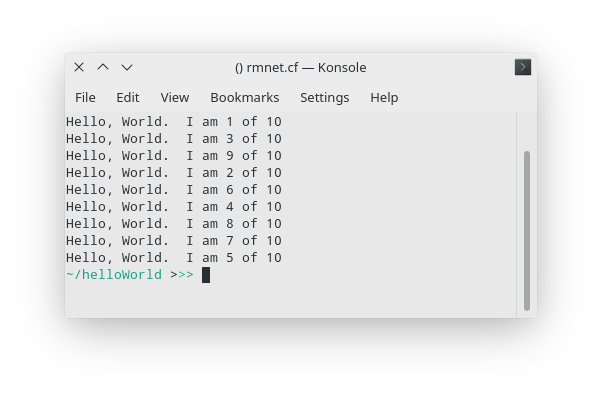
\includegraphics[width=\linewidth]{CITY3111/bitmaps/figure_15.png}
    \caption{Screenshot of successful Hello World execution}
    \label{figure_15}
\end{figure}

Upon running the script, I am presented with a printout from each node specifying its identification number (`rank') and its location in the cluster as a while (where the cluster size is represented by `size' in code). This run confirms the cluster is operational and concludes my experimentation with the `hello world' program.
\vfill\break

\textbf{\sffamily{Initial functioning code: Revision 5, problems with effort shrink and other areas to improve}}

Before I commence a discussion on the evolution of my program over its development timeline, please note that the final code will be placed in full within Appendix β if you wish to bypass this section and read it directly.

Revision five marks the first working and compiled version of my program. To begin distributing the source code, I will checkout copies to each node. In future, to update the cluster all I will need to do is recompile from source on my laptop and update the subversion (SVN) folder on each node.

\begin{figure}[H]
    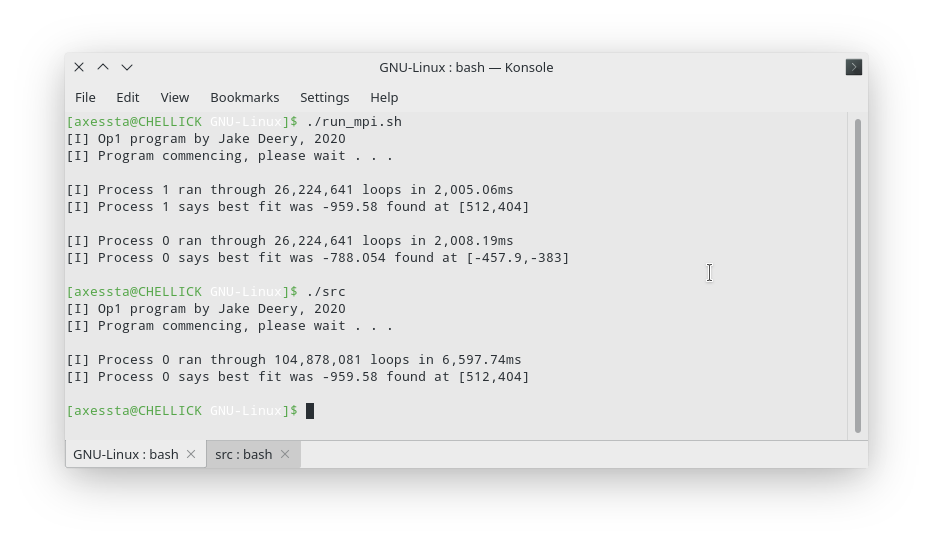
\includegraphics[width=\linewidth]{CITY3111/bitmaps/figure_16.png}
    \caption{Screenshot of initial functioning test run}
    \label{figure_16}
\end{figure}

This initial revision of my software appears to work in principle, with both of my development machine's CPU cores spinning up to 100\% for the 5 700 ms in which the program runs for. The inceptive promise is, however, dampened by several issues both in terms of functionality and semantics.

Addressing firstly the functionality of my program, the overall verbosity isn't yet up to the standards I wish it to be. Currently, I am only being presented with statistics on each node's effort, timings, best fit value and co-ordinates. While this data is entirely acceptable and I don't need anything else in terms of content, what will not be acceptable as I add more nodes is the lack of combined metrics.

The semantic issues that don't necessarily affect program functionality but can be defined as bugs are related to the underlying mechanics of my software. For some reason which I will need to investigate and rectify, my program is reporting conflicting total effort values. When running under a single node, my cluster appears to take 104 878 081 program loops to complete its search while two nodes combine for a computational effort of 52 449 282 program loops, somewhere around half of the total effort. This means approximately half of the search space is not being addressed in the latter case. Additional inspection shows that this effect is exponential.

\textbf{\sffamily{Progress report: Revision 10, functional improvements and object-oriented programming}}

This portion of my implementation represents a step towards my target program, mainly due to the functional improvements and improved coherence and efficiency in the underlying codebase. A majority of the codebase has been rewritten to facilitate better message-passing using the MPI\_Send and MPI\_Recv methods.

\begin{figure}[H]
    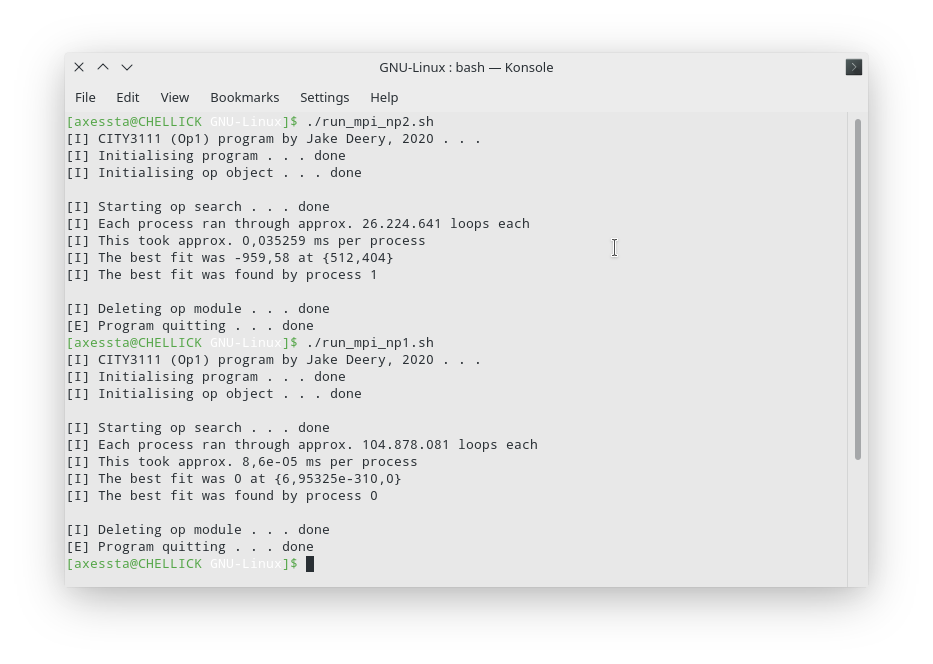
\includegraphics[width=\linewidth]{CITY3111/bitmaps/figure_17.png}
    \caption{Screenshot of improved program test run}
    \label{figure_17}
\end{figure}

The resultant program is now much cleaner in its verbosity and has a slightly smaller memory footprint (2 612 KiB for r5 vs. 2 608 KiB for r10) thanks to its conversion from a C program (procedural) to a C++ one (objective). Despite these improvements, existing semantic bugs are unresolved and new bugs have appeared.

The most obvious issue presents itself when looking at the single-node execution, where the apparent best fit is zero at an indeterminate set of co-ordinates. This is likely due to the fact that I put a lot of the program's code inside a set of if statements that change how each node behaves (specifically, I have defined a master/slave architecture against how I initially planed to).

To resolve this, I will need to amalgamate the thought process I was using up to revision five with the improvements and concepts I have learned since. As well as this, I will need to start addressing the semantic issues that have plagued the project up until this point.

\textbf{\sffamily{Approaching completion: Revision 30, a stable codebase and additional functional improvements}}

Since making my software object-oriented, I have taken advantage of new techniques at my disposal to further improve the program's efficiency, including making greater use of private variables and function arguments to make modifying variables better and to create a better, more readable flow of code.

\begin{figure}[H]
    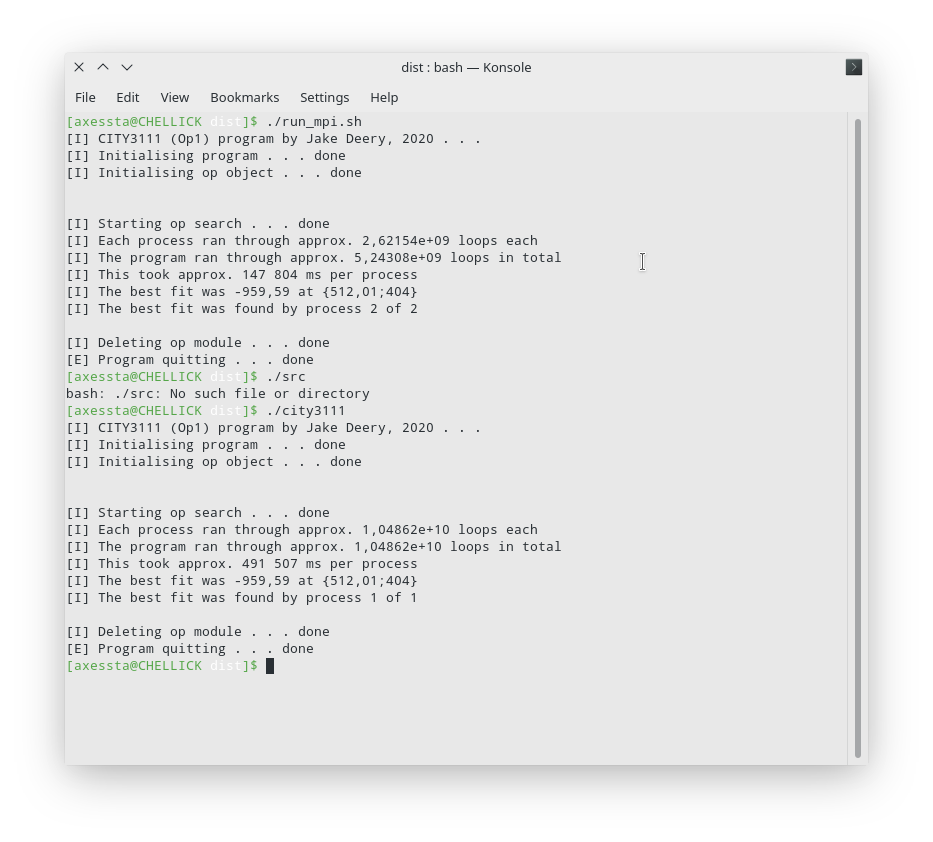
\includegraphics[width=\linewidth]{CITY3111/bitmaps/figure_18.png}
    \caption{Screenshot of latest program test run}
    \label{figure_18}
\end{figure}

One example of improvements I have made in the last 20 revisions is the precision float I have added, which now makes it possible to define the precision of my search without needing to modify the object itself, as I was before. Another functional change I have made is further increases in verbosity. Before, to calculate the total effort across all nodes, one needed to multiply the printed value by the number of nodes. I have now added a line that approximates the value with a view to make it an accurate representation in the near future.

In a semantic sense, the program has only improved marginally. A singular node is now once again capable of running the process single-handedly, however I am going to need to take a major look into the problem space issues and address them head-on before the next major milestone is reached.

\textbf{\sffamily{Final software revision: A change in search-space bounding and better total effort counting}}

I have finally reached a point in my implementation where I can demonstrate a codebase I am happy to say is at a stage of prototyping that is stable and bug-free enough to submit to the next stage -- a review of results and discussion on improvements to be made for production.

\begin{figure}[H]
    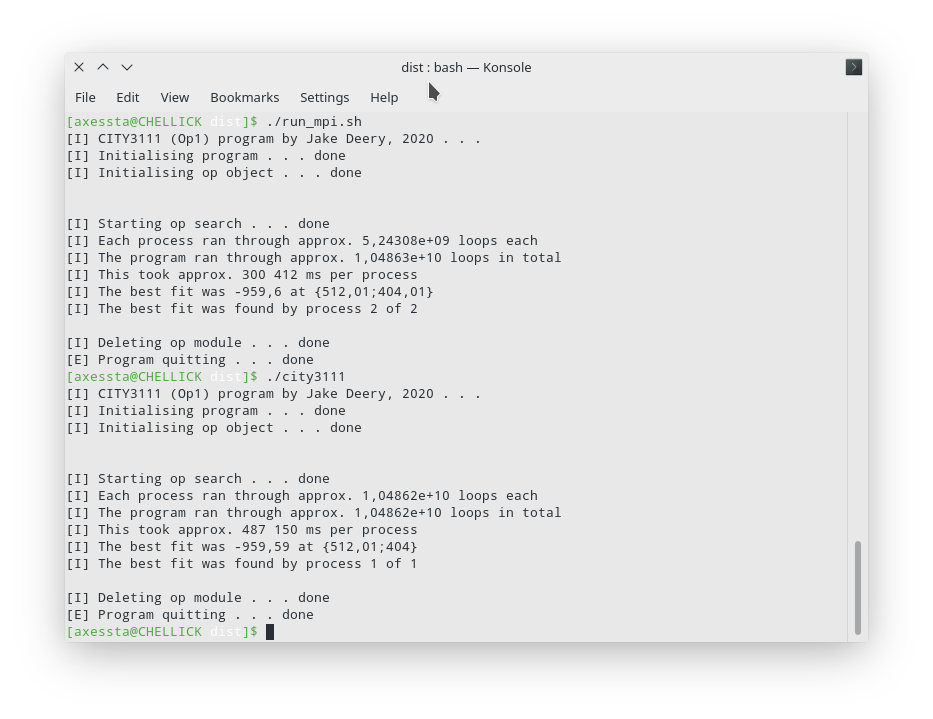
\includegraphics[width=\linewidth]{CITY3111/bitmaps/figure_19.png}
    \caption{Screenshot of final program test run}
    \label{figure_19}
\end{figure}

At a functional level, there have been no fundamental changes whatsoever to my software. Semantically however, there are two major changes to the software and how it is addressing the problem which are of interest.

Firstly, rather than approximating the computational effort using the master node's effort value as a basis, each node now communicates its effort counters back for amalgamation. This provides a better overview of any effort shrink as it takes into account the fact that the last node in the cluster will typically have a slightly smaller problem area due to overlap avoidance techniques.

\begin{figure}[H]
    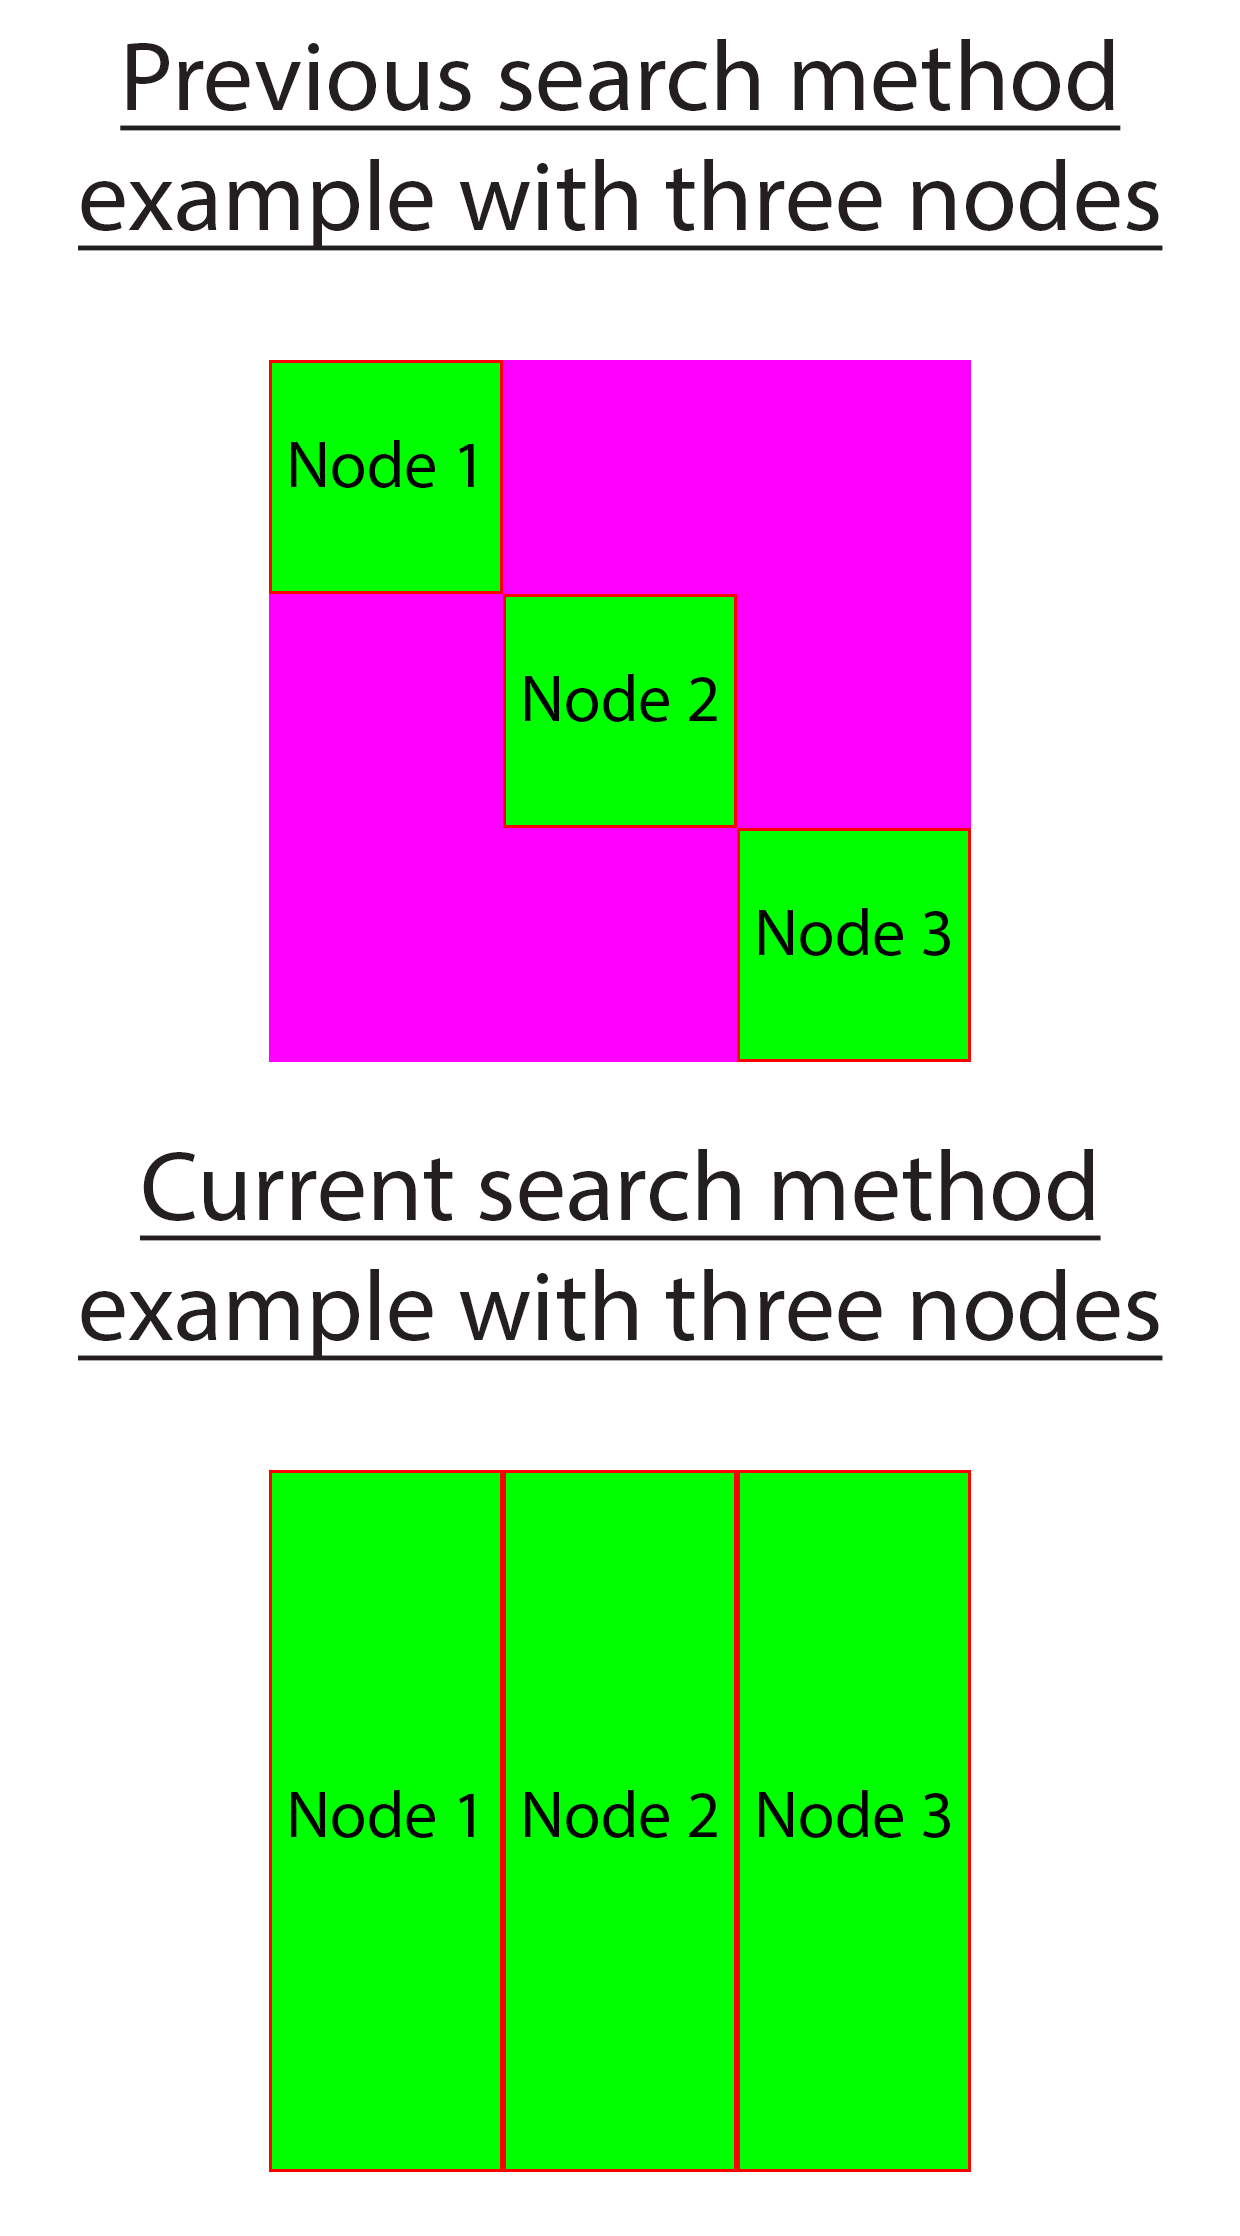
\includegraphics[width=\linewidth]{CITY3111/bitmaps/figure_20.png}
    \caption{Demonstration of problem area solution for effort creep}
    \label{figure_20}
\end{figure}

Secondly, the method I was previously using to search the problem area has been improved to cover the complete area and reduce (although not completely halt) effort creep. The problem ended up being a programming error on my behalf that was easily fixed. My initial implementation was using square search areas in which the bonding areas for the X-axis were also being used on the Y-axis.

This resulted in a set of squares that, when viewed on a 2D plot, appeared to be mirror copies moving from the top-left to bottom-right (assuming a UV plot where \{-512,-512\} is in the top-left). The solution I used ended up being to lock the Y-axis search to cover the entire search range from -512 to 512.

This results in a stripe-search pattern when viewed on a 2D plot which gives each node roughly the same problem areas. This also reduces problem shrink to a much lower and more manageable change which should give a more scientific result. Content on the program's ability to perform the benchmarking I need it to, I am now to proceed onto Chapter 5, where I will gather results from the cluster, analyse their meaning and discuss future work I could perform to improve my cluster or its software.
